\documentclass[xcolor=dvipsnames]{beamer} 
\usecolortheme[named=Blue]{structure} 
\usetheme[height=10.5mm]{Rochester} 
\setbeamertemplate{items}[ball] 
\setbeamertemplate{blocks}[rounded][shadow=true] 
\setbeamertemplate{navigation symbols}{} 
\usepackage{bm}
\usepackage{rotating}
\usepackage{graphicx}
\usepackage{multirow}
\usepackage{hyperref}
\usepackage{textcomp}
\usepackage{upquote}
\usepackage[absolute,overlay]{textpos}
\newenvironment{reference}[2]{%
  \begin{textblock*}{\textwidth}(#1,#2)
      \footnotesize\it\bgroup\color{red!50!black}}{\egroup\end{textblock*}}
%\graphicspath{ {/home/ben/PhD/Armidale_Updates/2014_03_14/Figures/} }
\begin{document}

\begin{frame} %1
% \frametitle{Addressing Common Challenges in Spatial Modeling of Ecologies and Environments}
%\begin{center}
\textbf{\huge Introduction to R}\\
a language and environment for statistical computing and graphics %
%\end{center}

\begin{figure}

\includegraphics[width = 0.35\textwidth]{/home/ben/Intro_to_R/Introductory_Slides_Source/Images/R_logo.png}
\end{figure}
\small Ben R. Fitzpatrick\\
\tiny PhD Candidate, Statistical Science, Mathematical Sciences School, Queensland University of Technology
\newline
\begin{columns}
\begin{column}{3cm}
\tiny 0000-0003-1916-0939
\end{column}
\begin{column}{3cm}
\tiny github.com/brfitzpatrick/
\end{column}
\begin{column}{3cm}
\tiny @benrfitzpatrick
\end{column}
\end{columns}
\end{frame}

\begin{frame} 
\frametitle{}
\begin{itemize}
\item Please sit in groups
\newline
\item Anyone who has used R before please spread yourselves around 1 per group
\newline
\item so I can help you all more efficiently could the people using MacOS please sit together and the people using Windows also please site together
\end{itemize}
\end{frame}

\begin{frame} 
\frametitle{What is R?}
\begin{itemize}
\item R is a language and environment for statistical computing and graphics
\newline
\item R similar to the S language and environment 
\newline
\item R is Free and Open Source Software
\newline
\item R will compile and run on most popular operating systems e.g. MS Windows, MacOS, UNIX, FreeBSD \& GNU+Linux
\end{itemize}
\end{frame}

\begin{frame} 
\frametitle{Why Use R?}
\framesubtitle{R is Free in the Sense of Free Speach \& Free Beer}
\begin{itemize}
\item chance are if you have a `modern' computer you will be able to install R on it
\newline
\item unlike software with paid licensing models you can use R anywhere free of charge
\newline
\item you are free to modify and extend R provided you acknowledge the contributions of those who have gone before you
\end{itemize}
\end{frame}

\begin{frame} 
\frametitle{Why Use R?}
\framesubtitle{R is Popular with a Large \& Steadily Growing User Base}
Subsequently packages have been written for R that implement a wide range of statistical analyses.
Furthermore, more packages and functionality are continually being added and active forums exist on which to seek and find help.
\begin{figure}
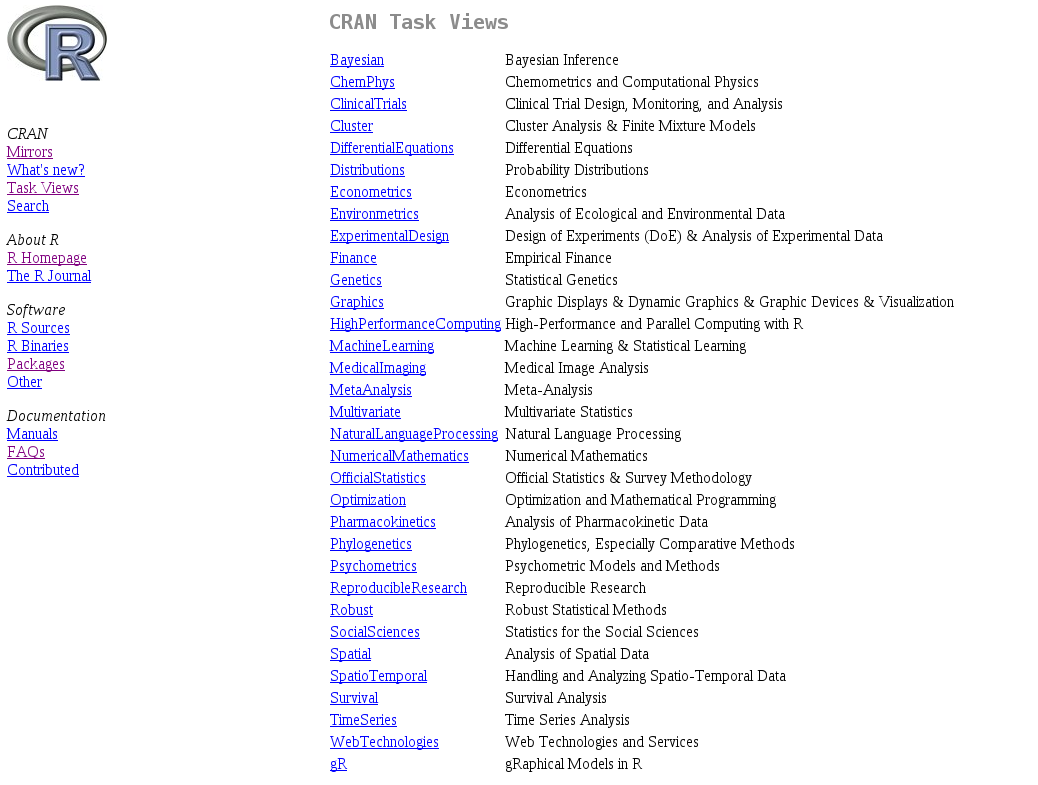
\includegraphics[height = 0.7\textheight]{/home/ben/Intro_to_R/Introductory_Slides_Source/Images/CRAN_Task_Views.png}
\end{figure}

\end{frame}

\begin{frame} 
\frametitle{Why Use R?}
\framesubtitle{R has powerful graphics authoring capabilities}

\begin{figure}
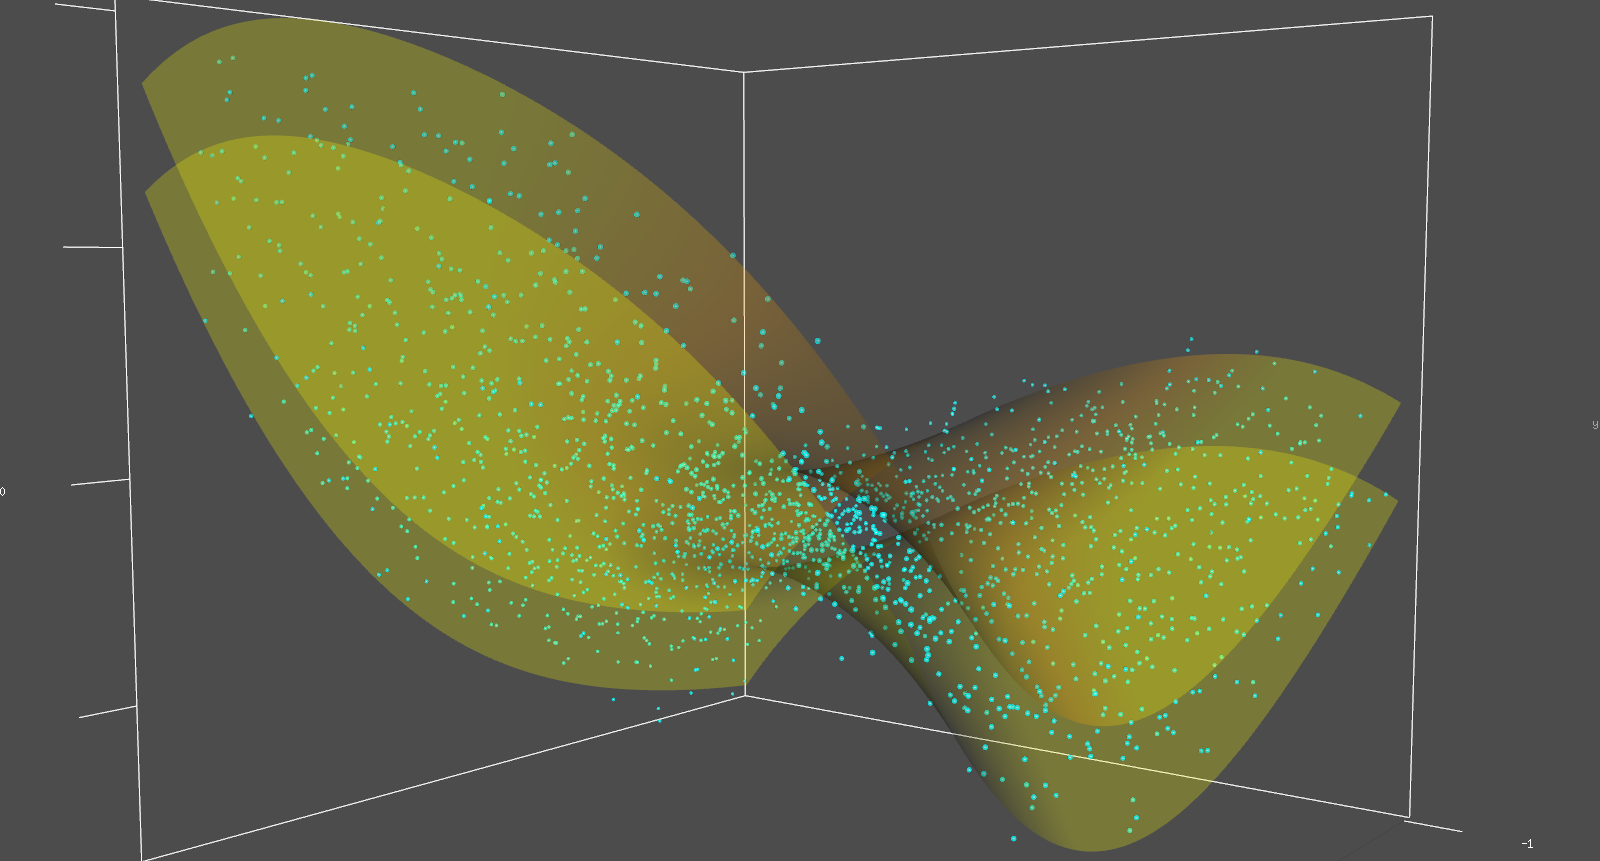
\includegraphics[width = 0.95\textwidth]{/home/ben/Intro_to_R/Introductory_Slides_Source/Images/179.png}
\end{figure}

\tiny 3D visualisation produced with the `rgl' R package

\end{frame}

\begin{frame} 
\frametitle{Why Use R?}
\framesubtitle{R has powerful graphics authoring capabilities}

\begin{figure}
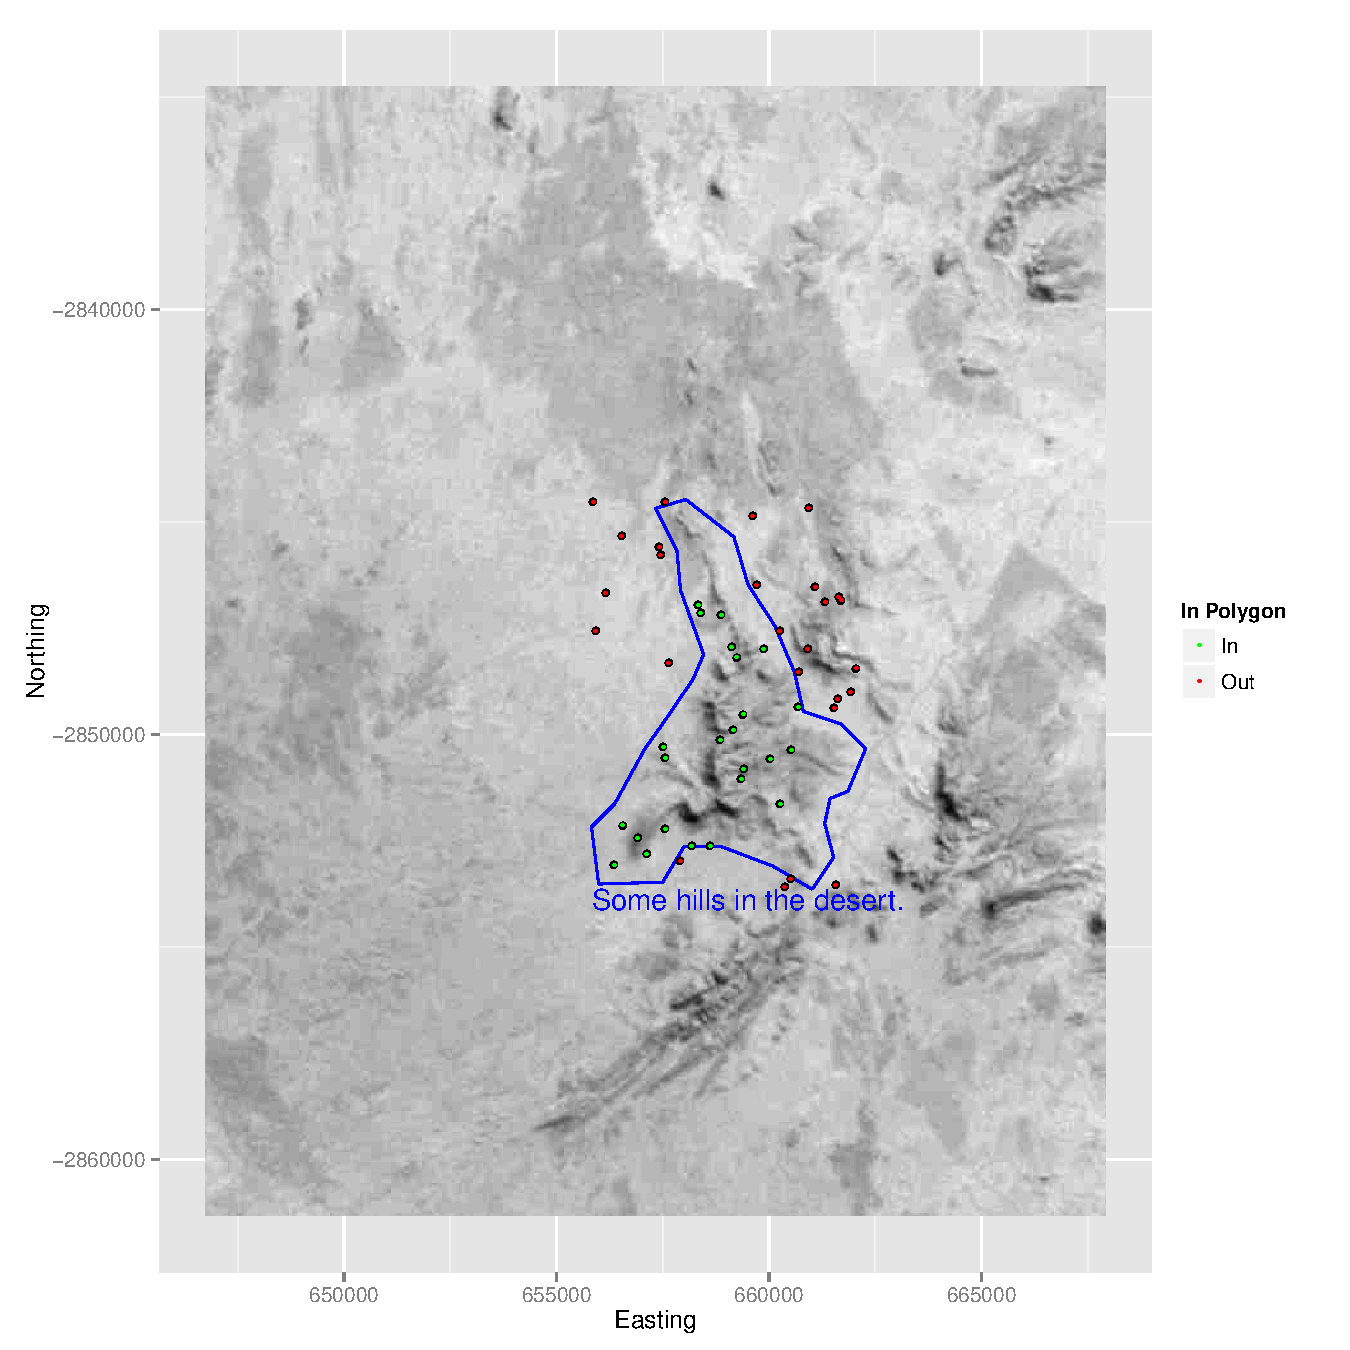
\includegraphics[width = 0.85\textheight]{/home/ben/Intro_to_R/Introductory_Slides_Source/Images/desert.pdf}
\end{figure}

\tiny Geospatial Visualisation produced with the R packages `raster' \& `ggplot2'

\end{frame}

\begin{frame} 
\frametitle{Why Use R?}
\framesubtitle{R has powerful graphics authoring capabilities}
\begin{center}
\begin{figure}
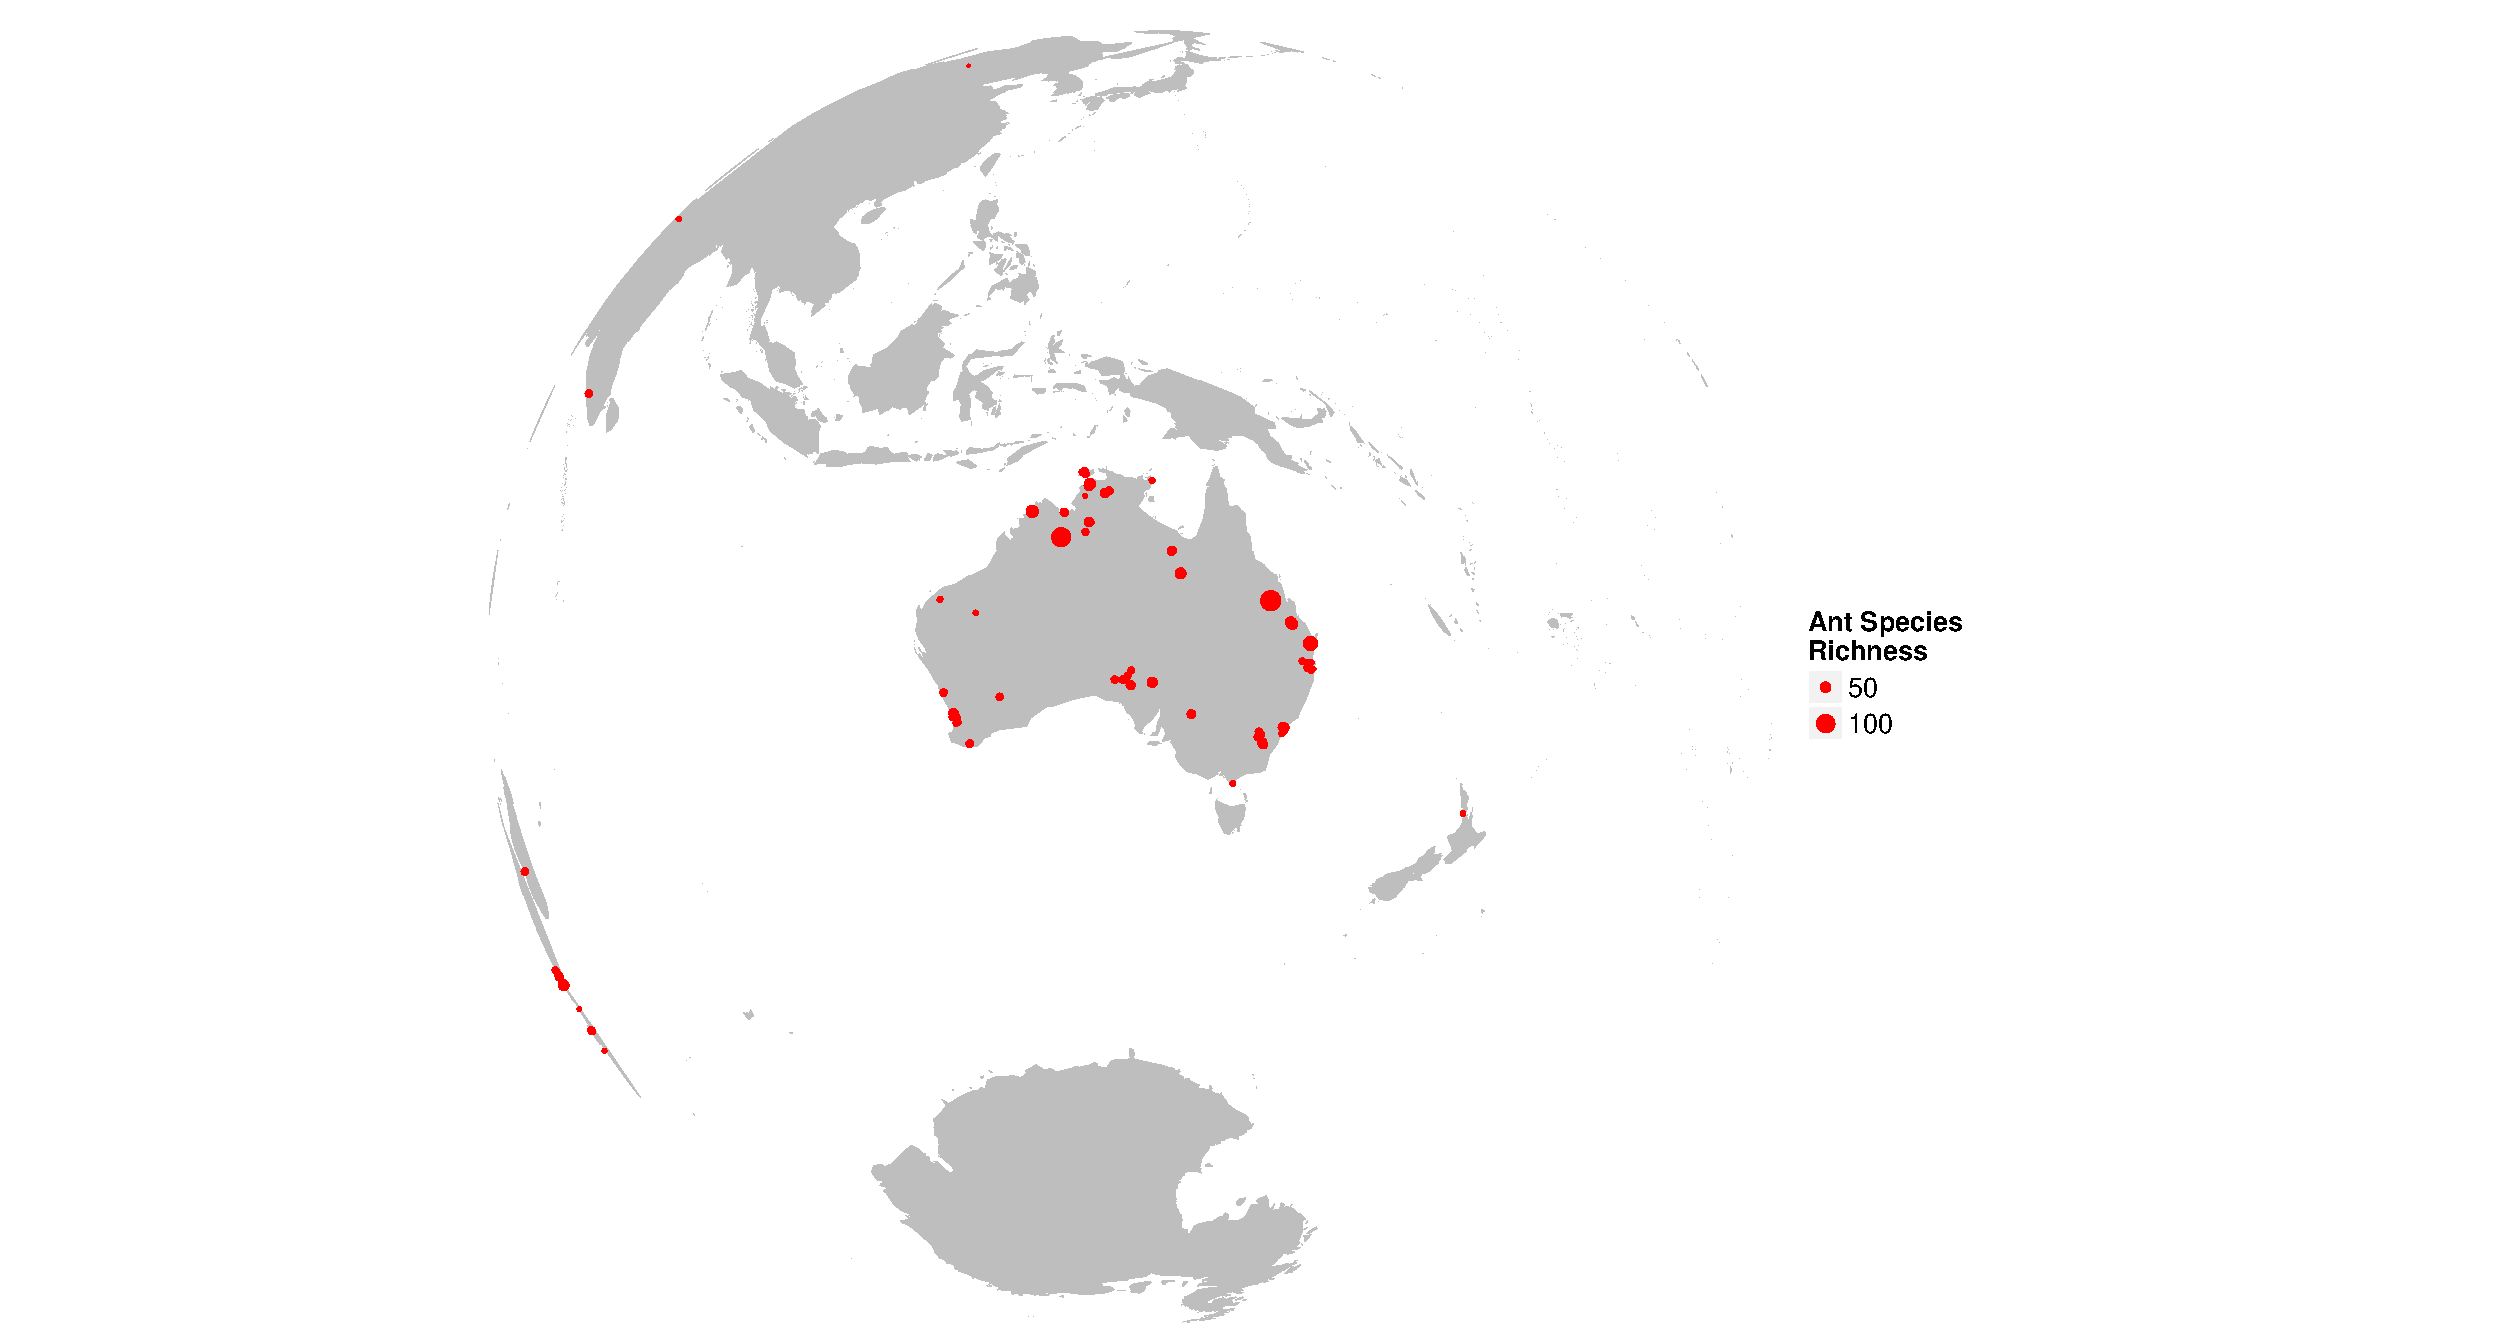
\includegraphics[height = 0.75\textheight]{/home/ben/Intro_to_R/Capstone_Collaborative_Exercise/Capstone_Slides_Source/Images/Ant_Sp_Rich_Globe_Map.pdf}
\end{figure}
\end{center}
\tiny Geospatial Visualisation produced with the R packages `maps \& `ggplot2'

\end{frame}

\begin{frame} 
\frametitle{Ways to Use R}
\begin{itemize}
\item via a command line interface e.g. PowerShell or Terminal
\newline
\item via the default GUI clients for MS Windows \& Mac OS
\newline
\item via one of many Integrated Development Environments that either have been exclusively written for R or have R language modes e.g. \begin{itemize}
 \item RStudio
 \item Tinn-R
 \item Sublime Text
 \item Atom
 \item Emacs Speaks Statistics
 \item ...
\newline
 \end{itemize}

\item remotely i.e. submitting R scripts to a sever (e.g. HPC facility) to execute
\end{itemize}
\end{frame}

%\begin{frame}
%\frametitle{Ways to Use R:}
%\framesubtitle{In a termial e.g. on MS Windows}
%\begin{figure}
%\includegraphics[width = 0.35\textwidth]{~/Presents_Intro_to_R/Introductory_Slides_Source/Images/R_Console_MacOS.png}
%\end{figure}
%\end{frame}

\begin{frame}
\frametitle{Ways to Use R:}
\framesubtitle{In a termial e.g. on Mac OS}
\begin{figure}
\includegraphics[width = \textwidth]{/home/ben/Intro_to_R/Introductory_Slides_Source/Images/R_Console_MacOS.png}
\end{figure}
\end{frame}

\begin{frame}
\frametitle{Ways to Use R:}
\framesubtitle{In a termial e.g. on GNU+Linux}
\begin{figure}
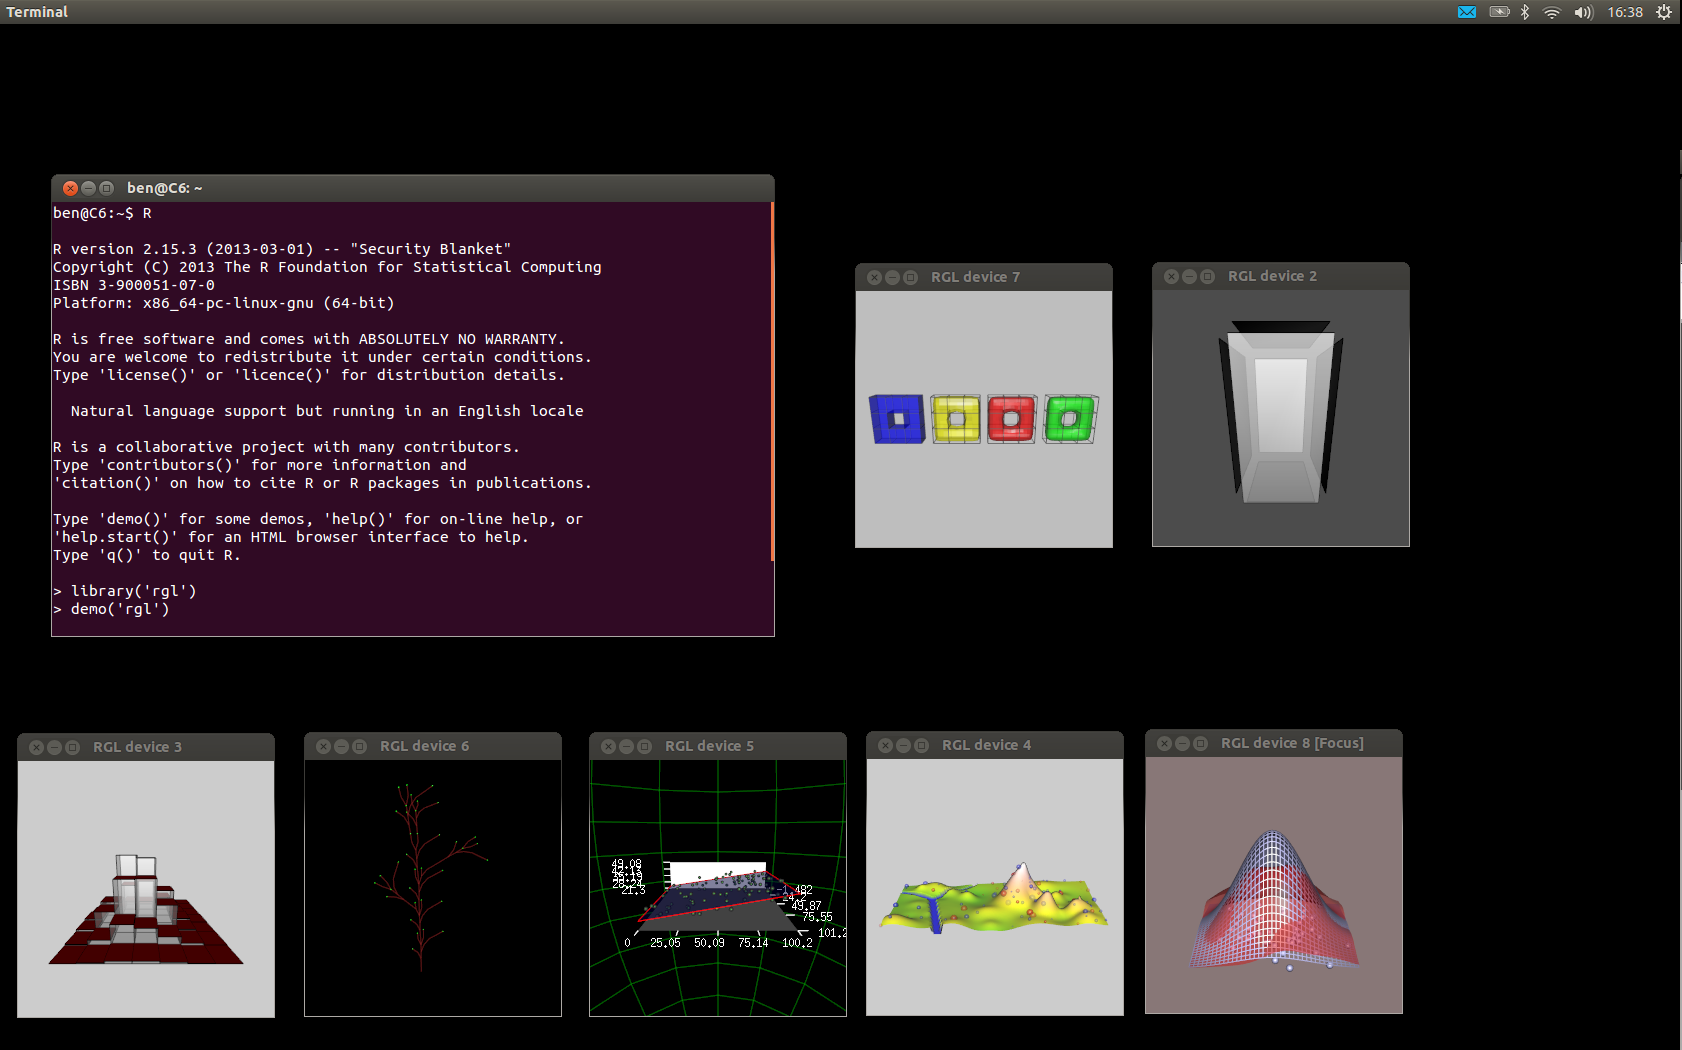
\includegraphics[width = \textwidth]{/home/ben/Intro_to_R/Introductory_Slides_Source/Images/R_in_Ubuntu_Terminal_2.png}
\end{figure}
\end{frame}

\begin{frame}
\frametitle{Ways to Use R:}
\framesubtitle{Default Windows Client}
\begin{figure}
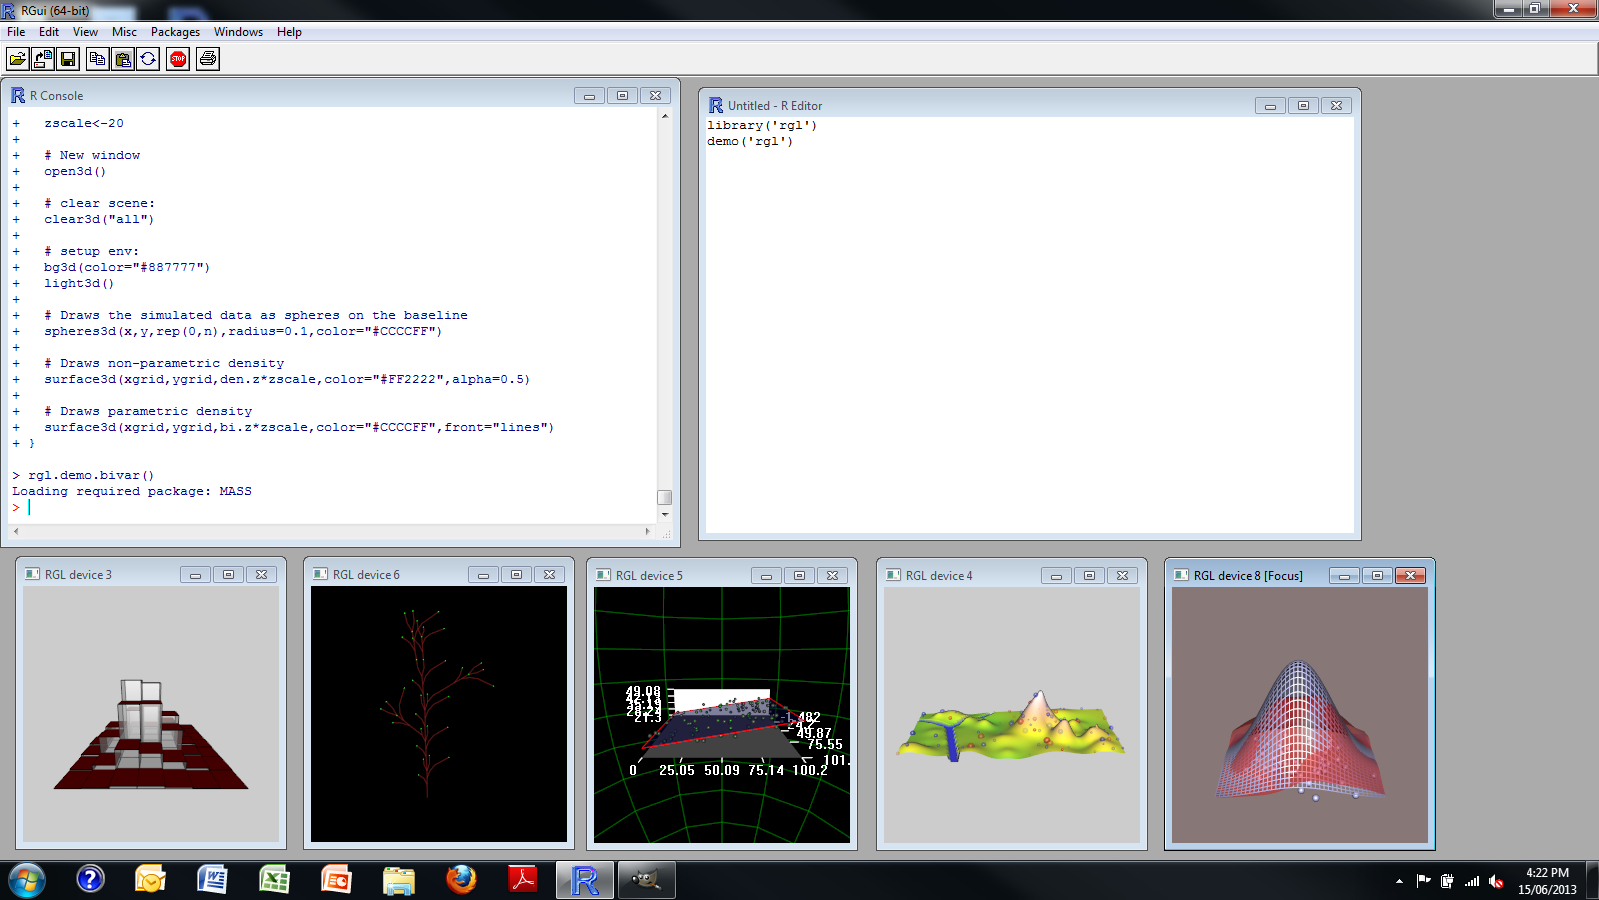
\includegraphics[width = \textwidth]{/home/ben/Intro_to_R/Introductory_Slides_Source/Images/R_on_Windows.png}
\end{figure}
\end{frame}

\begin{frame}
\frametitle{Ways to Use R:}
\framesubtitle{Tinn-R Integrated Development Environement}
\begin{figure}
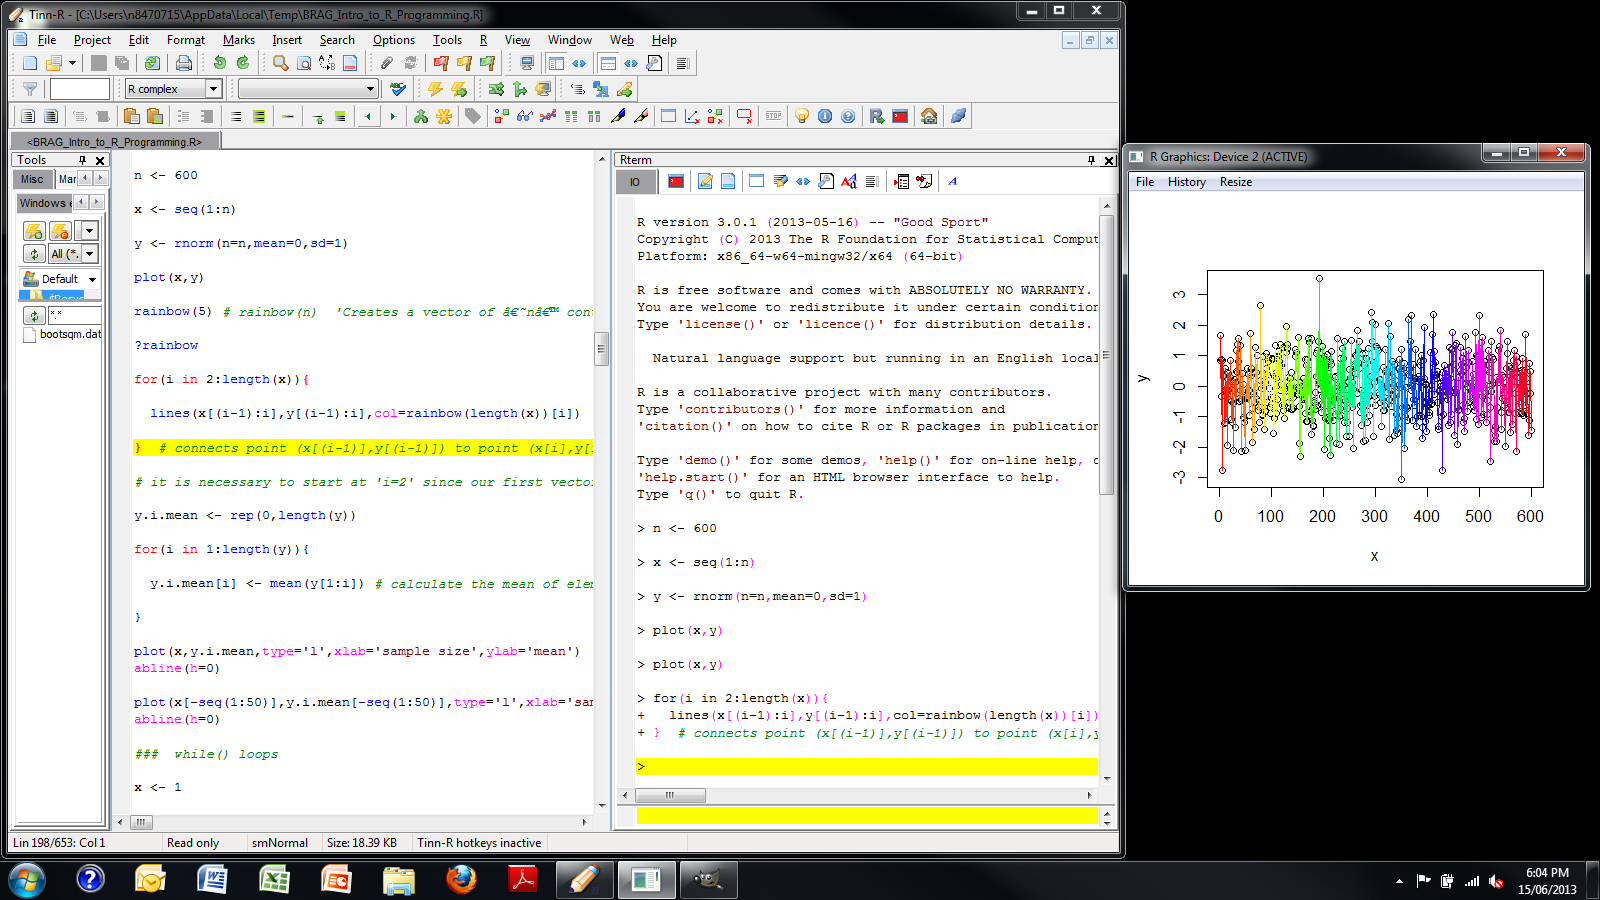
\includegraphics[width = \textwidth]{/home/ben/Intro_to_R/Introductory_Slides_Source/Images/TinnR.png}
\end{figure}
\end{frame}

\begin{frame}
\frametitle{Ways to Use R:}
\framesubtitle{Emacs Speaks Statistics Integrated Development Environement}
\begin{figure}
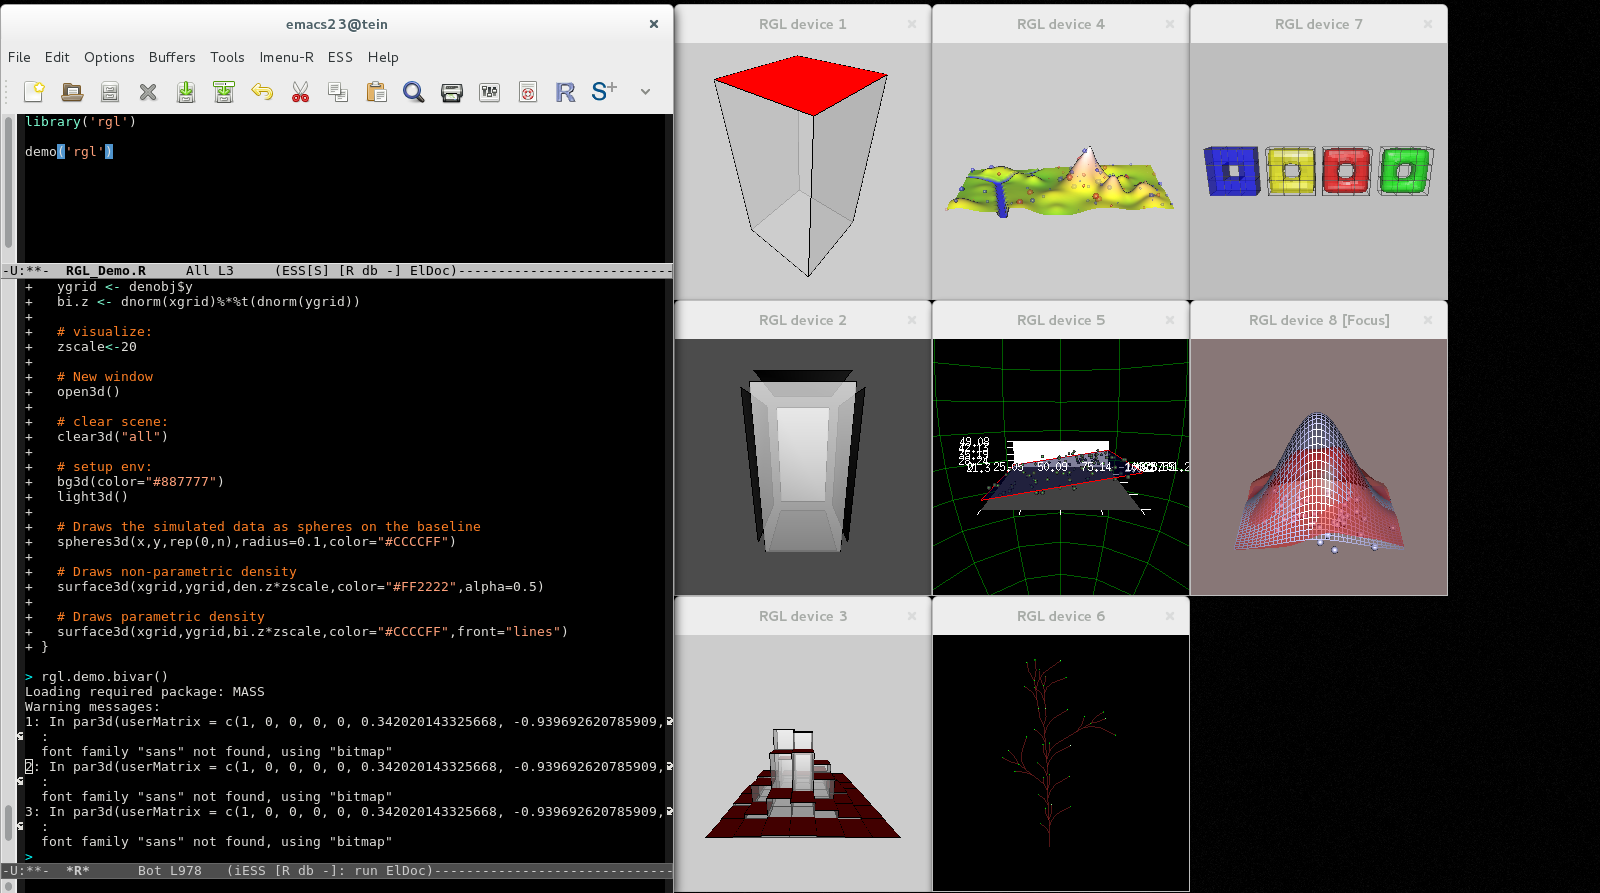
\includegraphics[width = \textwidth]{/home/ben/Intro_to_R/Introductory_Slides_Source/Images/R_ESS_Debian_GNU_Linux.png}
\end{figure}
\end{frame}

\begin{frame}
\frametitle{Ways to Use R:}
\framesubtitle{RStudio Integrated Development Environement}
\begin{figure}
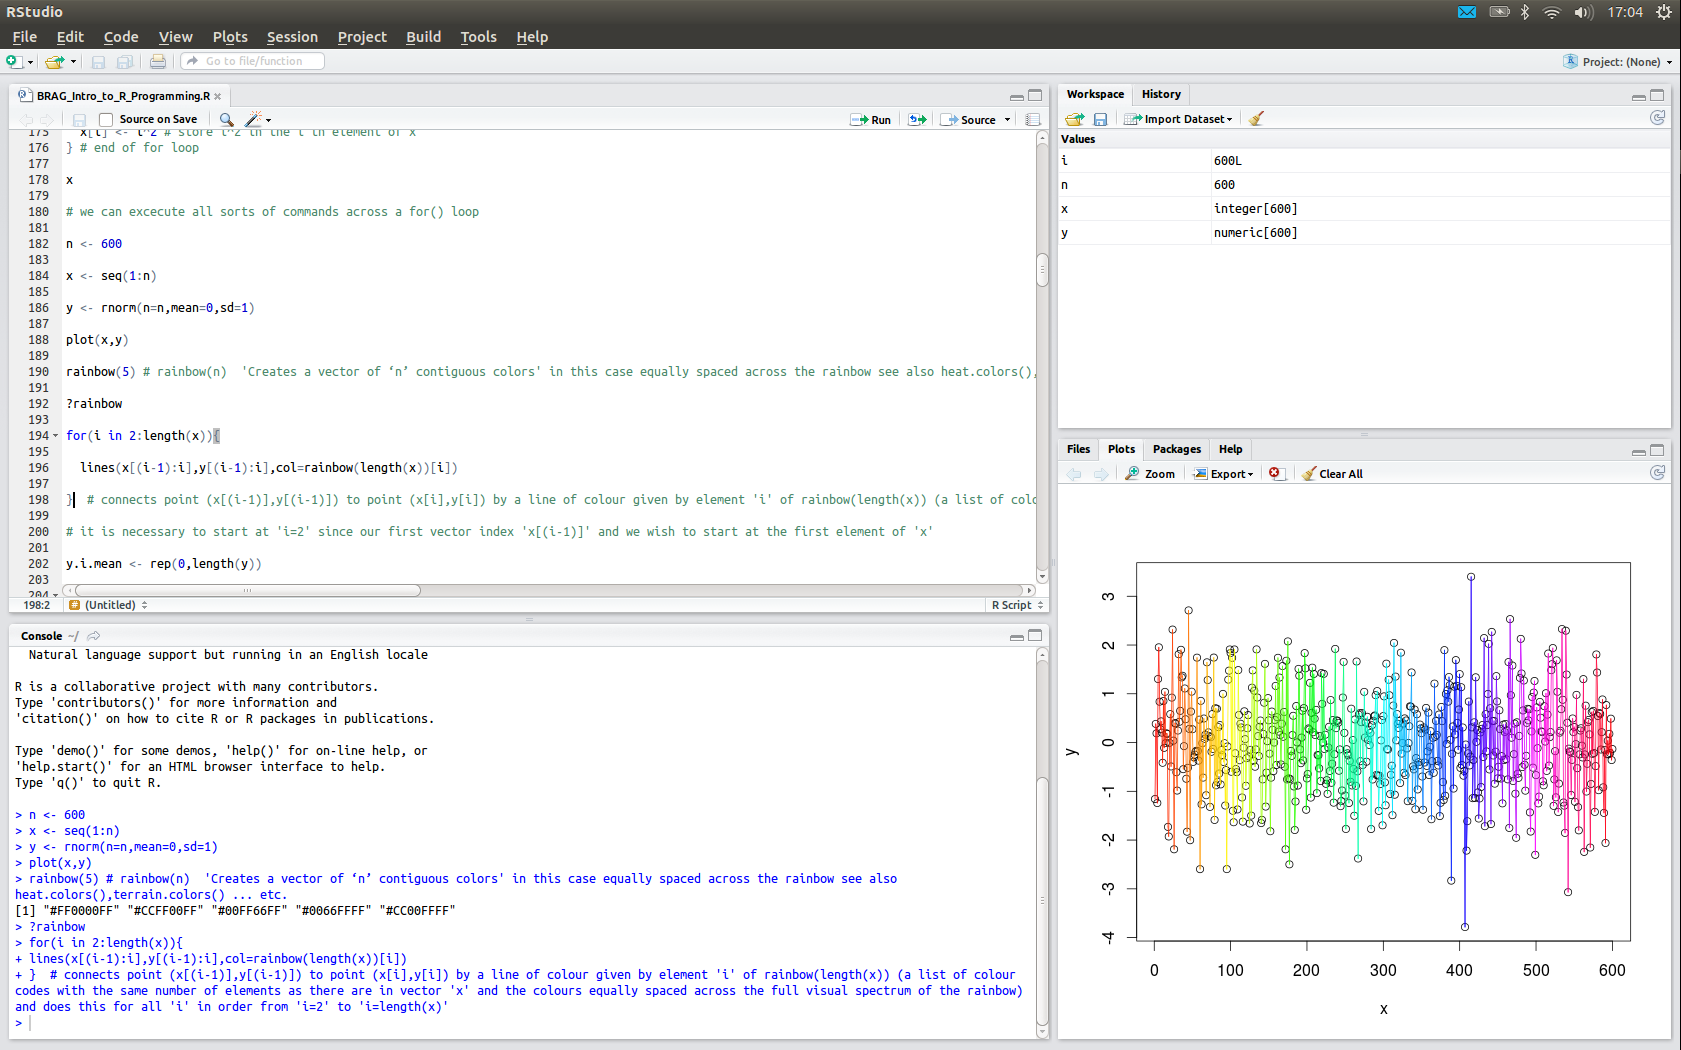
\includegraphics[width = \textwidth]{/home/ben/Intro_to_R/Introductory_Slides_Source/Images/RStudio_R.png}
\end{figure}
\end{frame}

\begin{frame}
\frametitle{For this course I encourage you to use the RStudio IDE}
Because:...
\begin{itemize}
\item it's comparatively intuitive and easy to learn
\newline
\item feature rich
\newline
\item available for most major operating systems (MS Windows, Mac OS, various flavours of GNU+Linux)
\newline
\end{itemize}
However, if you have already begun your journey learning R using a different IDE and wish to continue to use it please feel free to do so, provided you feel confident to open and execute .R files with this IDE.

\end{frame}

\begin{frame}
\frametitle{The Plan}
\framesubtitle{Feel free to use this time to pursue something that interests you}
Course organised into 5 instructory modules and one extended, collaborative exercise.
\newline
\newline
Module: \begin{enumerate}
\item Introduction to R \& RStudio  
\item Graphics with the R package `ggplot2'
\item Linear Modelling in R
\item Programming in R
\item Version Control for solo \& collaborative source code management with Git \& GitHub
\item Capstone Collaborative Exercise
\end{enumerate}

\end{frame}

\begin{frame}
\frametitle{Module 1}
\framesubtitle{Introduction to R \& RStudio}
\begin{block}{Key Learning Outcomes}
Familiarisation with \begin{itemize}
\item Command Line Computing
\item RStudio Integrated Development Environment
\item Commands and arguments
\item Common Object Classes in R
\item Assigning values to Objects
\item Saving \& Loading R Workspaces
\item R Base Graphics
\item Data Input
\end{itemize}
\end{block}
\end{frame}

\begin{frame}[fragile]
\frametitle{Module 2}
\framesubtitle{Graphics with `ggplot2'}
\begin{block}{Key Learning Outcomes}
The key concepts \& mechanics of the plotting with the Grammar of Graphics$^1$ inspired `ggplot2': \begin{itemize}
\item the mechanics of the \begin{verbatim} ggplot( ) \end{verbatim} command
\item the concept of aesthetic mapping
\item plotting geometries
\item scales
\item faceting
\item saving plots
\end{itemize}
\end{block}

\tiny $^1$ Leland Wilkinson, \textit{The Grammar of Graphics}, Statistics and Computing. Springer, 2nd edition, 2005.
\end{frame}

\begin{frame}
\frametitle{Module 3}
\framesubtitle{Linear Modelling in R}
\begin{block}{Key Learning Outcomes}
\begin{itemize}
\item read data into R from an external file
\item fit linear regression models
\item produce \& examine model diagnostics
\item plot data along with predictions of model and associated uncertainty
\item conduct stepwise variable selection
\item produce summary statistics for model
\end{itemize}
\end{block}
\end{frame}

\begin{frame}
\frametitle{Module 4}
\framesubtitle{Programming in R}
\begin{block}{Key Learning Outcomes}
Writing:
\begin{itemize}
\item conditional statements
\item loops
\item functions
\newline
\end{itemize}
Solving problems by writing programs
\end{block}
\end{frame}

\begin{frame}
\frametitle{Module 5}
\framesubtitle{Version Control with Git \& GitHub}
\begin{block}{Key Learning Outcomes}
Understand:
\begin{itemize}
\item motivations for managaing a coding project via a version control system
\item fundamentals of Git \& GitHub: \begin{itemize}
  \item local and remote repositories
  \item developing multiple versions of the same file
  \item combining disparate versions of the same file
  \item returning to previous version of a file without loosing the current version
  \item collaboratively editing files
  \end{itemize}
\end{itemize}
\end{block}
\end{frame}

\begin{frame}
\frametitle{Module 6}
\framesubtitle{Collaborative Exercise}
\begin{block}{The Plan}
Form small groups and collaboratively explore and analyse some data on ant species richness around the globe.
Please re-use as much of the code from the preceeding exercises as you would like to.
\end{block}

\begin{block}{Key Learning Outcomes}
Practise and in doing so consolidate the skills you have learned over this course
\end{block}
\end{frame}

\begin{frame}
\frametitle{If you're already familiar with R}
\framesubtitle{Feel free to use this time to pursue something that interests you}
You could:
\begin{itemize}
\item Visit the GitHub directory for this course and pick a code file you like to start working through \url{https://github.com/brfitzpatrick/Intro_to_R}
\item See how far you can get through the incrementally harder maths/programming problems at \url{https://projecteuler.net/}
\item pursue your own project work
\end{itemize}
tuning in occasionally for the sections that interest you.
\newline
\newline
I'll need to focus on delivering the course but I'll try to check in with you peridocially throughout the next 2.5 days.
\end{frame}


\begin{frame}
\frametitle{Let's begin}
\begin{center} \huge Please open RStudio \end{center} 
\end{frame}



\begin{frame} 
\frametitle{Image Credits}
R Foundation, from http://www.r-project.org - Originally from http://developer.r-project.org/Logo/Rlogo.svg, modified to simpler SVG format.
%
\end{frame}


\end{document}
